\section{\rqone: Does FSE~2026 Replicate at Fixed Sample Size?}
\label{sec:rq1}

This section evaluates the four FSE claims (Section~\ref{sec:posterior})
at the original paper's own lens: strategies compared after acquiring the
same \emph{number} of configurations. Table~\ref{tab:rq1} aggregates the
per-corpus outcomes; Figure~\ref{fig:heatmap} shows the full outcome
matrix, including the cost-indexed outcomes of Section~\ref{sec:rq2}.

\begin{table}[t]
  \centering\small
  \caption{\rqone{} outcomes per corpus at fixed sample size. H1: KW test
  on posterior-risk distributions ($\alpha{=}.05$; arrows give
  Benjamini--Hochberg corrected counts where they differ). Best
  (confidence): \srs{} has the highest integrated posterior confidence.
  Best (risk): \srs{} has the lowest median posterior risk. H5: \srs{}
  risk significantly below \randomS.}
  \label{tab:rq1}
  \begin{tabular}{@{}lrrrrr@{}}
    \toprule
    Corpus & Scopes & H1 differ & \srs{} best (conf.) & \srs{} best (risk) & H5 \srs{}$<$\randomS \\
    \midrule
    FSE artifact & 7 & 7/7 & 5/7 & 4/7 & 6/7 \\
    x264 & 34 & 34/34 & 28/34 & 24/34 & 34/34 \\
    ENERGY & 220 & 212/220 & 12/220 & 22/220 & 52 $\to$ 42/220 \\
    WORKLOAD & 359 & 341/359 & 59/359 & 72/359 & 84 $\to$ 70/359 \\
    Linux & 21 & 21/21 & 0/21 & 0/21 & 5 $\to$ 1/21 \\
    LCBench & 210 & 154 $\to$ 144/210 & 1/210 & 0/210 & 0/210 \\
    \midrule
    Total & 851 & $\approx$95\% & --- & --- & --- \\
    \bottomrule
  \end{tabular}
\end{table}

\begin{figure}[t]
  \centering
  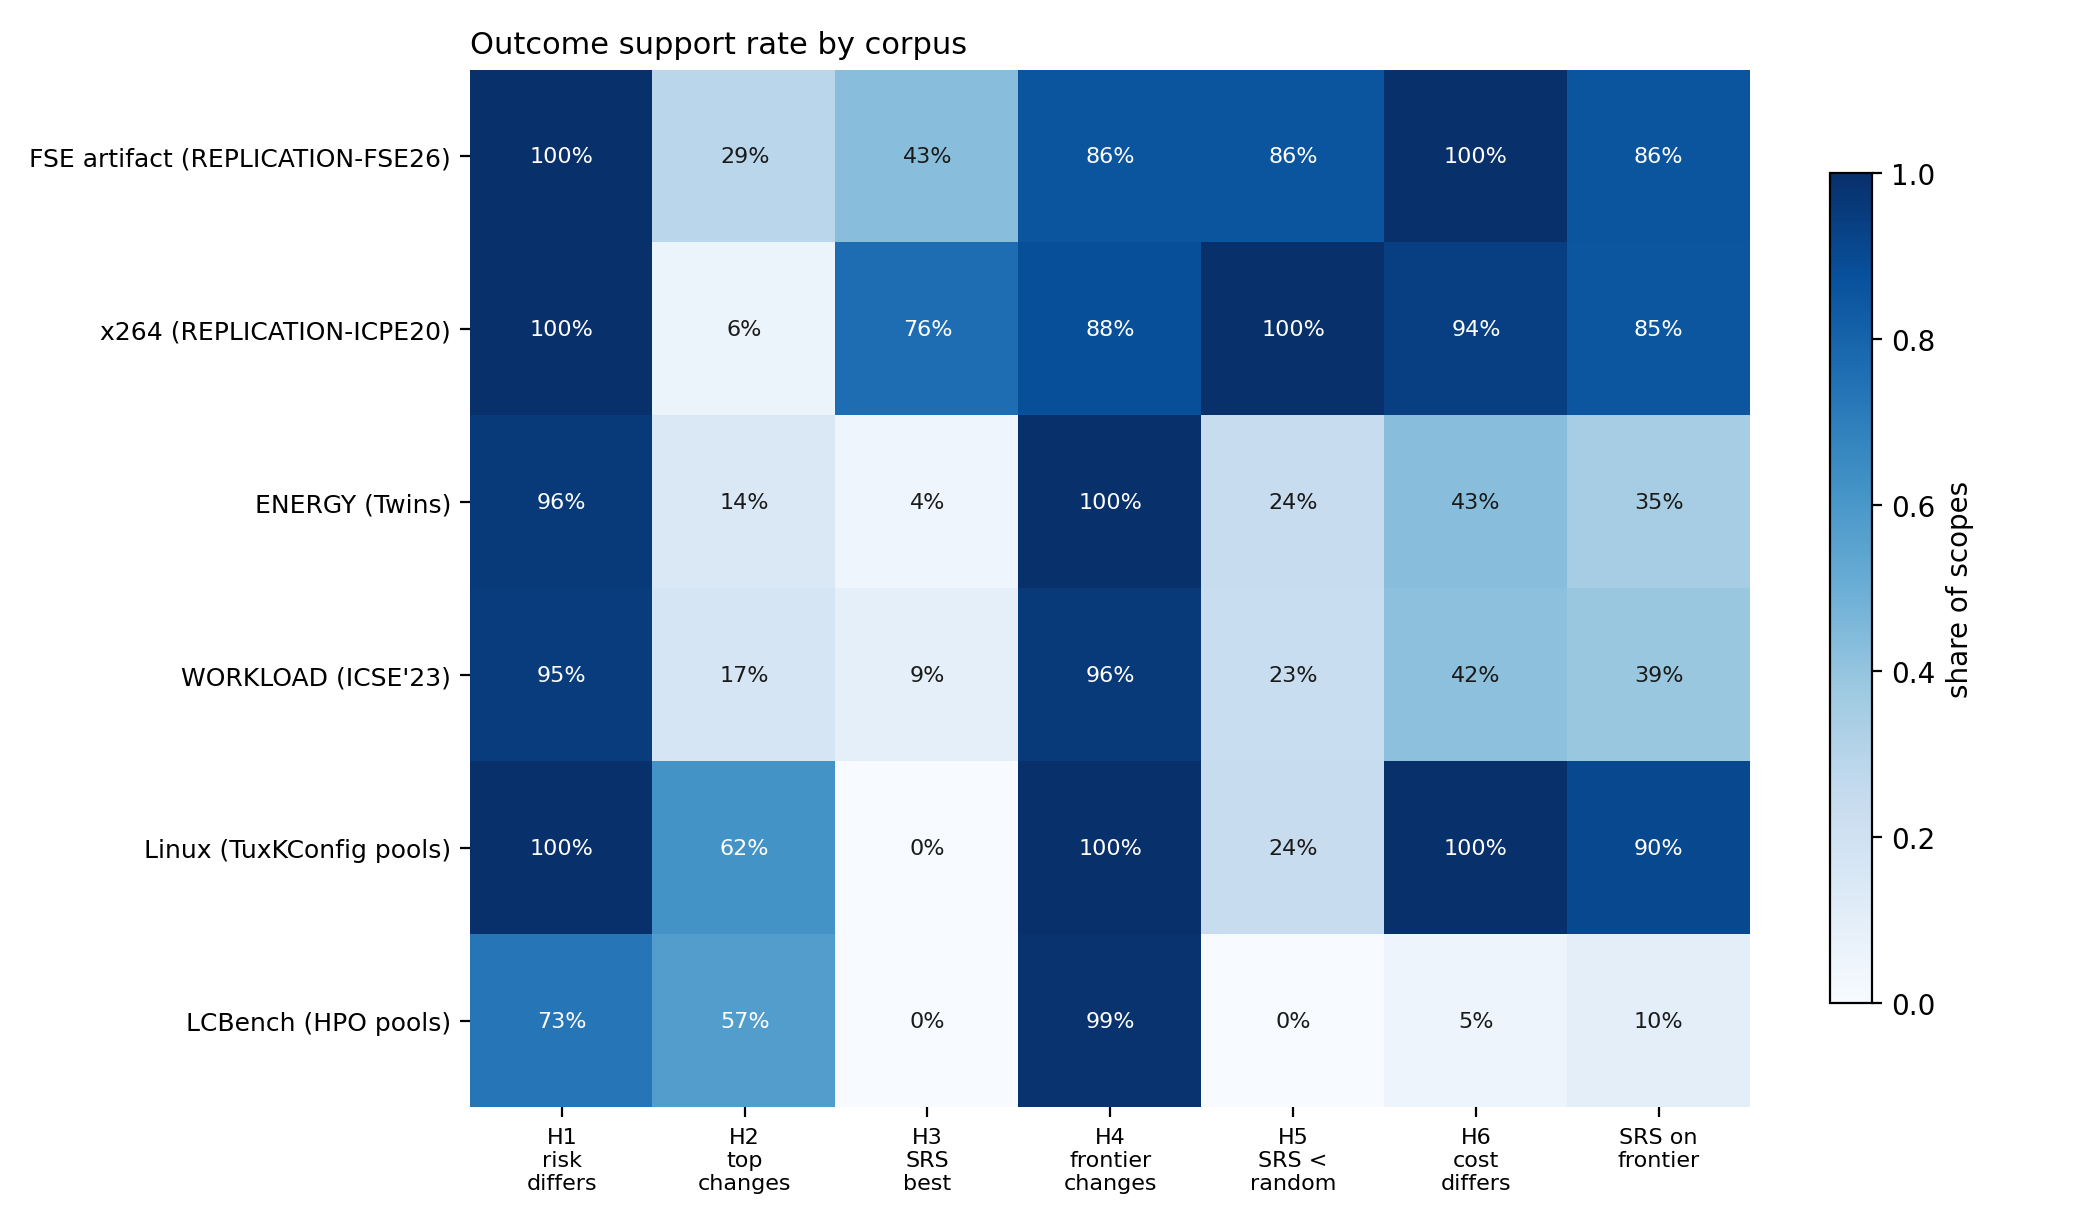
\includegraphics[width=.94\linewidth]{figures/fig_synthesis_heatmap.png}
  \caption{Outcome support rates by corpus (share of scopes; Linux row
  shows the full-protocol run). H1/H5/H6 are significance-based; H2--H4
  and frontier membership are decision rules
  (Section~\ref{sec:stats}).}
  \label{fig:heatmap}
\end{figure}

\subsection{RQ1.1: Discriminative power (C1)}

On the original artifact, all seven systems show significant differences
between the posterior-risk distributions of the five strategies,
reproducing C1 exactly. Figure~\ref{fig:polly} illustrates the
replication on Polly, the system the original paper singles out for
discussion, in the original paper's own visual idiom: per-strategy
posterior-risk distributions over 100 repetitions (left) and the
confidence discrepancy against the scenario-theoretic prior as the
accepted risk $\varepsilon$ varies (right). The strategies separate
cleanly---$t$-wise trades a deterministic, slightly higher risk for the
largest confidence gain at small $\varepsilon$, \srs{} and solver-based
sampling beat the prior, distance-based sampling falls below it. The
claim then generalizes to every corpus we add: 34/34 x264 contexts,
212/220 ENERGY scenarios, 341/359 WORKLOAD contexts, 21/21 Linux
release-level scopes, and 154/210 LCBench pools (144 after FDR
correction; the only corpus where correction moves the count). Overall,
posterior risk discriminates strategies in $\approx$95\% of 851
scopes---with no learner in the loop and across targets as different as
encoding time, energy, kernel size, and model accuracy.

\begin{figure}[t]
  \centering
  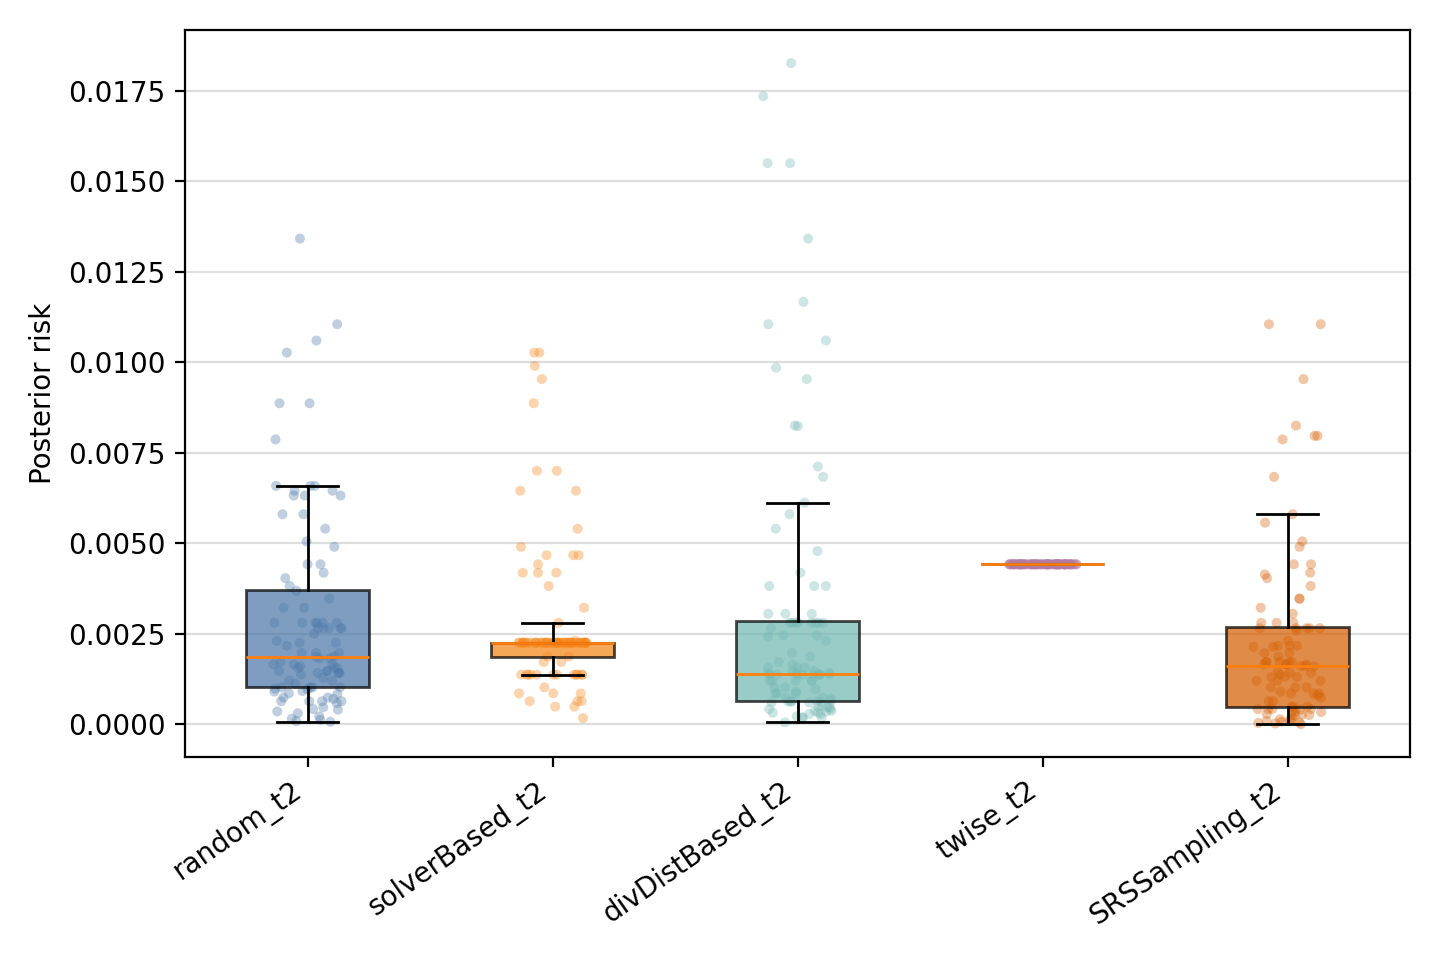
\includegraphics[width=.495\linewidth]{figures/fig_polly_risk.png}\hfill
  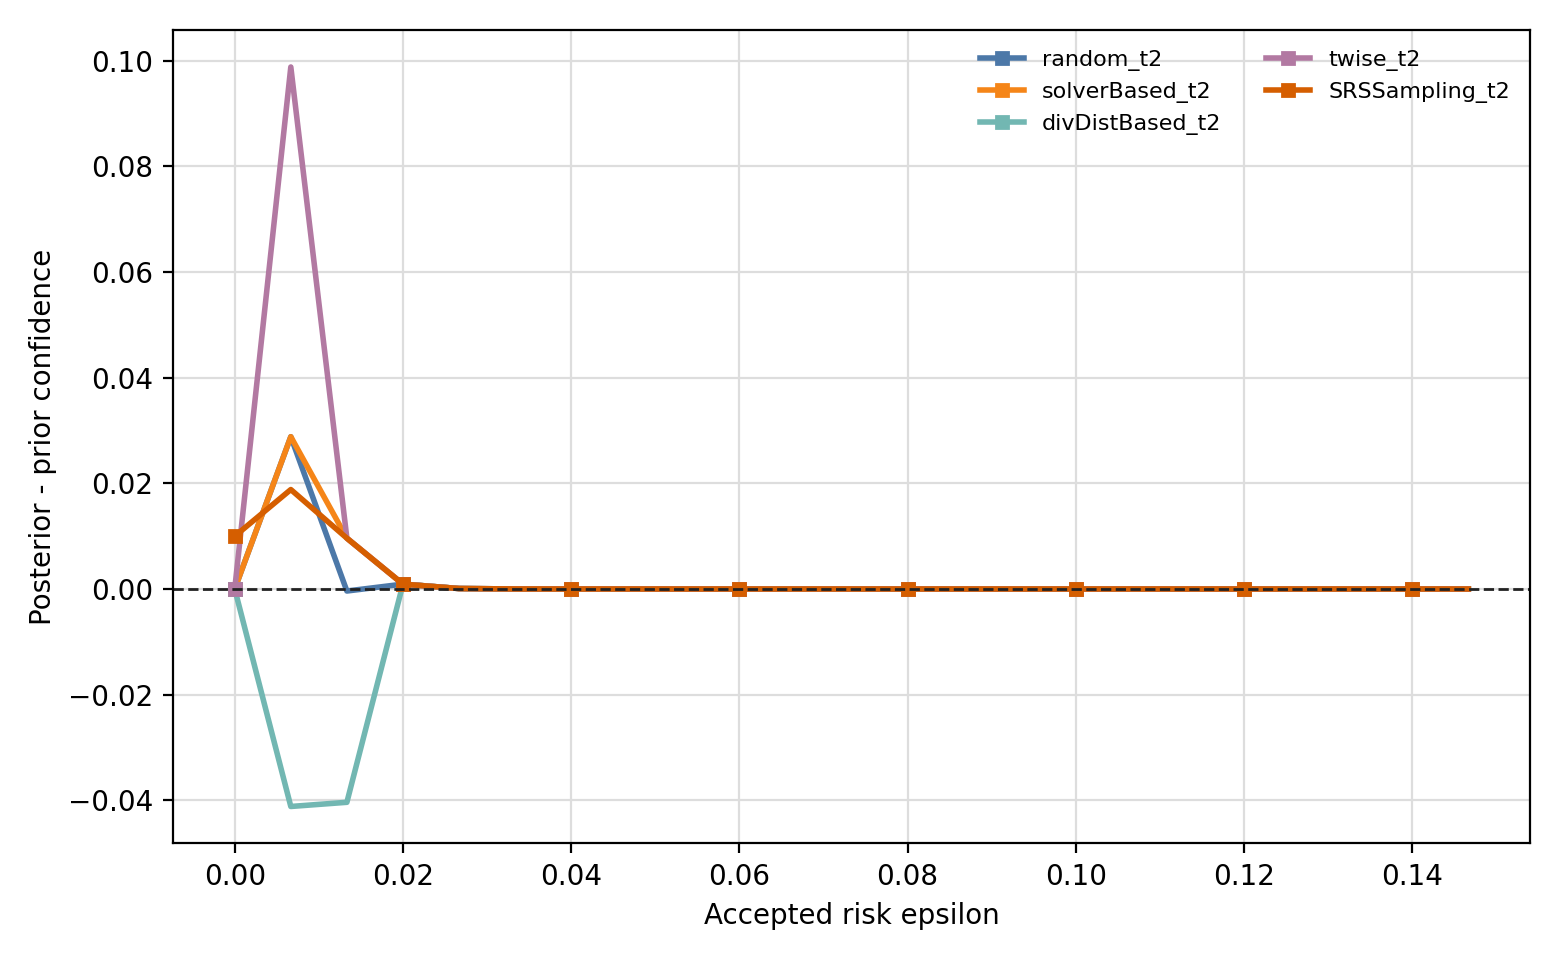
\includegraphics[width=.495\linewidth]{figures/fig_polly_confidence.png}
  \caption{Close replication on Polly (60{,}000 configurations, budget
  $t2=345$), in the visual idiom of \citet{weis2026risk}. Left:
  posterior-risk distributions per strategy (100 repetitions). Right:
  posterior minus prior confidence as a function of the accepted risk
  $\varepsilon$ (positive: better guarantees than the random-sampling
  prior at the same size).}
  \label{fig:polly}
\end{figure}

\finding{Finding 1 (C1 replicates and generalizes). Posterior risk and
confidence discriminate sampling strategies in $\approx$95\% of 851
scopes across six corpora, robust to FDR correction. The FSE~2026
evaluation framework is sound and portable.}

\subsection{RQ1.2: Budget scaling (C4)}

For each (context, strategy) pair we check whether median posterior risk
is non-increasing (and integrated confidence non-decreasing) along the
budget grid; Table~\ref{tab:scaling} reports the share of cells where
this holds. On configurable-software corpora the FSE expectation holds
broadly: 100\% of x264 cells, 98\% of Linux cells, 81\% of WORKLOAD and
76\% of ENERGY cells (the generated families use small budgets where
single-seed deterministic strategies can be non-monotone). For \srs{}
specifically, scaling is perfect (100\%) on \emph{all}
configurable-software corpora. On LCBench, however, monotonicity degrades
to 65\% of cells overall and 49\% for \srs: on
hyperparameter-optimization pools, growing the sample does not reliably
tighten \srs's bound, because its recursive restriction can lock onto
hyperparameter regions whose accuracy plateau differs from where the
pool's true optimum lies.

\begin{table}[t]
  \centering\small
  \caption{RQ1.2, budget scaling: share of (context, strategy) cells
  whose guarantees improve monotonically along the budget grid (median
  risk non-increasing; integrated confidence non-decreasing), for all
  strategies and for \srs{} alone. The FSE artifact runs a single budget
  level and is not applicable.}
  \label{tab:scaling}
  \begin{tabular}{@{}lrrrr@{}}
    \toprule
    & \multicolumn{2}{c}{All strategies} & \multicolumn{2}{c}{\srs} \\
    \cmidrule(lr){2-3}\cmidrule(l){4-5}
    Corpus & risk $\downarrow$ & conf.\ $\uparrow$ & risk $\downarrow$ & conf.\ $\uparrow$ \\
    \midrule
    x264 & 100\% & 100\% & 100\% & 100\% \\
    ENERGY & 76\% & 77\% & 100\% & 100\% \\
    WORKLOAD & 81\% & 81\% & 100\% & 100\% \\
    Linux & 98\% & 100\% & 100\% & 100\% \\
    LCBench & 65\% & 65\% & 49\% & 54\% \\
    \bottomrule
  \end{tabular}
\end{table}

\finding{Finding 2 (C4 replicates within the population, cracks outside).
Guarantees improve monotonically with sample size for \srs{} on every
configurable-software corpus (100\% of cells), but only in 49\% of
LCBench cells---the first boundary condition.}

\subsection{RQ1.3: \srs{} superiority (C2)}

On the original artifact, \srs{} is significantly better than uniform
random in 6/7 systems (H5), has the highest integrated confidence in 5/7,
and the lowest median risk in 4/7---consistent with the original
finding that \srs{} is the strongest, though not uniformly dominant,
strategy. On x264 the replication is even stronger: significantly better
than random in 34/34 contexts, best integrated confidence in 28/34.
x264's budgets are $t$-wise-scale (dozens to hundreds of samples),
matching the original protocol. Table~\ref{tab:ranks} summarizes the
fixed-size strategy ranking on both replication corpora: \srs{} is the
top-ranked strategy on both (mean rank 1.6 of 5, and 1.1 of 7), with
distance-based sampling a consistent second.

\begin{table}[t]
  \centering\small
  \caption{RQ1.3--1.4, fixed-size strategy ranking on the replication
  corpora: mean rank by median posterior risk across contexts at the
  $t2$ budget (1 = lowest risk). Strategies absent from a corpus are
  marked ---.}
  \label{tab:ranks}
  \begin{tabular}{@{}lrr@{}}
    \toprule
    Strategy & FSE artifact (of 5) & x264 (of 7) \\
    \midrule
    \srs & \textbf{1.6} & \textbf{1.1} \\
    Diversified distance-based & 2.3 & 2.9 \\
    Uniform random & 3.0 & 3.3 \\
    Distance-based & --- & 4.3 \\
    $t$-wise & 4.1 & 4.4 \\
    Henard's diversified & --- & 5.1 \\
    Solver-based & 3.7 & 6.1 \\
    \bottomrule
  \end{tabular}
\end{table}

The claim does not travel further. On the generated families at small
budgets ($n{=}8$--$64$), \srs{} is best in only 5--20\% of scopes and
beats random significantly in $\approx$19\% (FDR-corrected);
space-filling strategies (\diShe, \pairwise) dominate. On Linux, \srs{}
is \emph{never} the best strategy at fixed size (0/21) and beats random
in only 1/21 scopes after correction; on LCBench it is best by
integrated confidence in a single pool (1/210) and never by risk. Anticipating
Section~\ref{sec:rq2}: the equal-spend experiment shows this is chiefly a
\emph{budget} effect---\srs's advantage over random grows from 4\% of
ENERGY scopes at $n8$-scale budgets to 77\% at $n64$-scale
(Figure~\ref{fig:equalspend}B)---which reconciles its dominance at the
original protocol's larger budgets with its weakness at ours.

\finding{Finding 3 (C2 replicates where FSE tested it; it is
budget- and domain-dependent). \srs{} superiority replicates fully on the
original systems and on x264 (34/34), fades at small budgets on the
generated families, and vanishes on Linux and LCBench (best in at most 1
of 231 scopes). The advantage requires budget to amortize.}

\subsection{RQ1.4: Solver unreliability (C3)}

Solver-based sampling ranks near the bottom on both corpora where it
participates (Table~\ref{tab:ranks}): mean median-risk rank 3.7 of 5
strategies on the FSE artifact and clearly worst, 6.1 of 7, on x264. On
the FSE artifact only $t$-wise ranks lower by median risk---but
$t$-wise's deterministic sample yields zero risk variance and hence high
confidence at small tolerances, whereas solver-based sampling combines
mediocre risk with high variance, matching the original paper's
characterization of unreliable guarantees. Its samples, drawn from a SAT
solver's biased enumeration order, systematically miss the performance
extremes that bounds require, echoing prior findings on solver bias
\citep{plazar2019uniform}.

\finding{Finding 4 (C3 replicates). Plain solver-based sampling remains
the least reliable strategy for guarantees on both corpora that include
it.}

\subsection{\rqone{} answer}

All four FSE claims replicate on the original artifact under exact data
reuse, and the framework-level claims (C1, C3) replicate on every
applicable corpus. The strategy-level claims (C2, C4) replicate within
the population the original study sampled from---configurable software at
$t$-wise-scale budgets---and degrade predictably outside it. No claim
reverses on the original systems. In replication terms: a successful
close replication, and a conceptual replication that maps the claims'
boundary conditions rather than refuting them.
